% version 1.00, date 07/03/16, auteur Mélissa Bignoux
\documentclass[asi]{picInsa}

%Pour le schéma d'architecture
\usepackage{etex}
\usepackage{tikz}
\usetikzlibrary{shapes,arrows,chains,backgrounds,fit}
%FIN Pour le shéma d'architecture


\DeclareGraphicsRule{*}{pdf}{*}{}
\usepackage{pdfpages}

%\usepackage{colortbl}
\usepackage{fancyhdr}
\usepackage{listings} 
\usepackage{mathrsfs}
\usepackage{url}
\usepackage{lmodern}
\usepackage{color}
\usepackage{xcolor}
\usepackage{wrapfig}
\usepackage{graphicx}
\usepackage{pdflscape}
\usepackage{longtable}
\usepackage{sectsty}
\usepackage{lastpage}
\usepackage{multirow}
\usepackage{float}
\usepackage{eso-pic}
\usepackage[french]{minitoc}
\usepackage[babel=true]{csquotes}
\usepackage{tikz}
\addto\captionsfrench{\def\tablename{Tableau}}
\usepackage{vocabulaireUnipik}
%\usepackage{../../ressources/Unipik/vocabulaire/vocabulaireEastpic}

\setcounter{secnumdepth}{4}
\setcounter{tocdepth}{4}
\newcommand{\ligneMaj}[3] {
	\rowcolor[gray]{0.55} \textbf{\textit{#1}} & #2  &  #3\\
	\hline
}
\newcommand{\ligneSup}[3] {
	\rowcolor[gray]{0.65} |\textunderscore \textbf{\textit{#1}} & #2  &  #3\\
	\hline
}
\newcommand{\ligneMed}[3] {
	\rowcolor[gray]{0.75} \hspace{0.25cm} |\textunderscore #1  & #2 & #3 \\
	\hline
}
\newcommand{\ligneSub}[3] {
	\rowcolor[gray]{0.85}  \hspace{0.5cm} |\textunderscore #1 & #2 & #3\\
	\hline
}
\newcommand{\ligneSubSub}[3] {
	\rowcolor[gray]{0.95}  \hspace{0.75cm} |\textunderscore #1 & #2 & #3\\
	\hline
}
\newcommand{\ligneTache}[3] {
	\hspace{1.00cm} |\textunderscore #1 & #2 & #3\\
	\hline
}
\title{\DSI{}}
\author{\Pierre} %à changer


\titreGeneral{\DCP}
\sousTitreGeneral{\nomEquipe}
\titreAcronyme{\DCPCourt}
\version{V1.00}
\titreDetaille{\DCPCourt\_D\_\nomEquipe\_\versionPrive}
\referenceVersion{\DCPCourt\_D\_\nomEquipe\_\versionPrive}
\auteurs{\Matthieu{} \& \Kafui{} \& \Melissa{} \& \Sergi{} \& \Michel{} \& \Pierre{}}
\destinataires{\nomEquipe, \nomClient{}}
\resume{Le présent document contient la présentation du \DCP{} \nomEquipe.}
\motsCles{\DCPCourt{}}
\natureDerniereModification{ }
\modeDiffusionControle{}

\begin{document}

\couverture{}

 \informationsGenerales{}
% version 1.00, date 29/02/16, auteur Michel Cressant
\begin{pagesService}
	\begin{historique}
		% nouvelles versions à rajouter AU-DESSUS en recopiant les lignes suivantes et en les modifiant :
		\unHistorique{1.00}{02/02/2016}{\Michel}{Création}{Toutes}

	\end{historique}

%        \begin{suiviDiffusions}
%
%            % On place ici les diffusions
%        	\unSuivi{1.00}{}{\nomEquipe{}}
%          
%          
%        \end{suiviDiffusions}

%%Signataires
        \begin{signatures}
	   \uneSignature{Vérificateur}{\RRS}{\Matthieu{}}{17/03/2016}{PGPic}
       \uneSignature{Validateur}{\CP{}}{\Sergi}{}{PGPic}
        \end{signatures}
	
	

	
	
\end{pagesService}


\tableofcontents

\setcounter{chapter}{0}


\chapter*{Introduction}
\label{intro}
% version 1.01 Date 24/03/2016	Auteur Mathieu Medici

\section*{Objet}
L'objectif de ce document est de présenter les principes et les procédures nécessaires à la mise en œuvre de la gestion des configurations prévue par la norme \isoNeufMilleUn.

\section*{Définition}

Le présent document établit les règles et la structure de la gestion des configurations qui doivent être suivies pendant toute la durée du \picCourt. Il contient :
\begin{itemize}
\item les règles de nommage;
\item la description des différents référentiels;
\item les règles spécifiques de \nomEquipe{};
\item la description de l'administration des configurations;
\item la description de la maîtrise des documents;
\item la description de la maîtrise des enregistrements;
\item les règles d'archivage.
\end{itemize}



\chapter*{Diagramme de séquence}
\label{diagrammeSequence}
% version 1.00, date 20/02/16, auteur Michel Cressant
La figure suivante (figure \ref{diagramme_sequence}) indique le déroulement du remplissage de la base de données via les fichiers csv.

\begin{figure}[H]
	\centering
	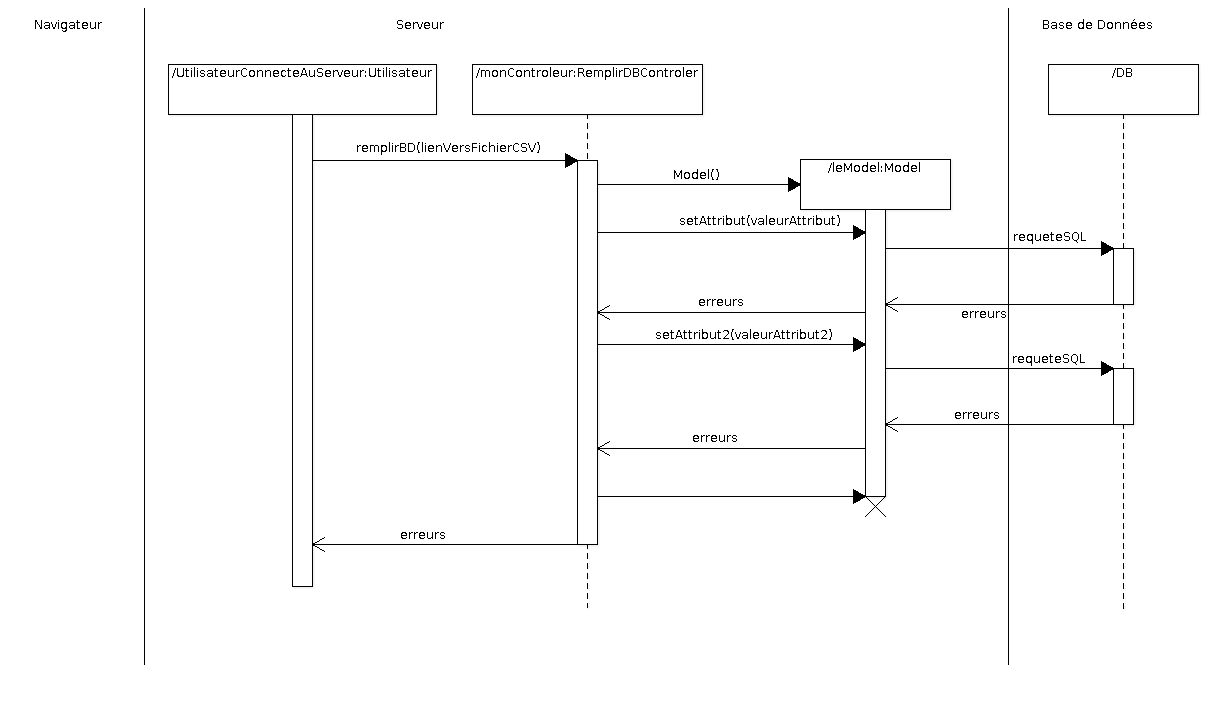
\includegraphics[scale=0.3]{diagrammeSequence/images/diagrammeSequence}
	\caption{Diagramme de séquence système pour le remplissage de la base de données}	
	\label{diagramme_sequence}
\end{figure}
	
%\newpage
La figure suivante (figure \ref{diagramme_sequence_2}) montre les actions effectuées lors d'une interaction entre l'utilisateur et l'IHM.

\begin{figure}[H]
	\centering
	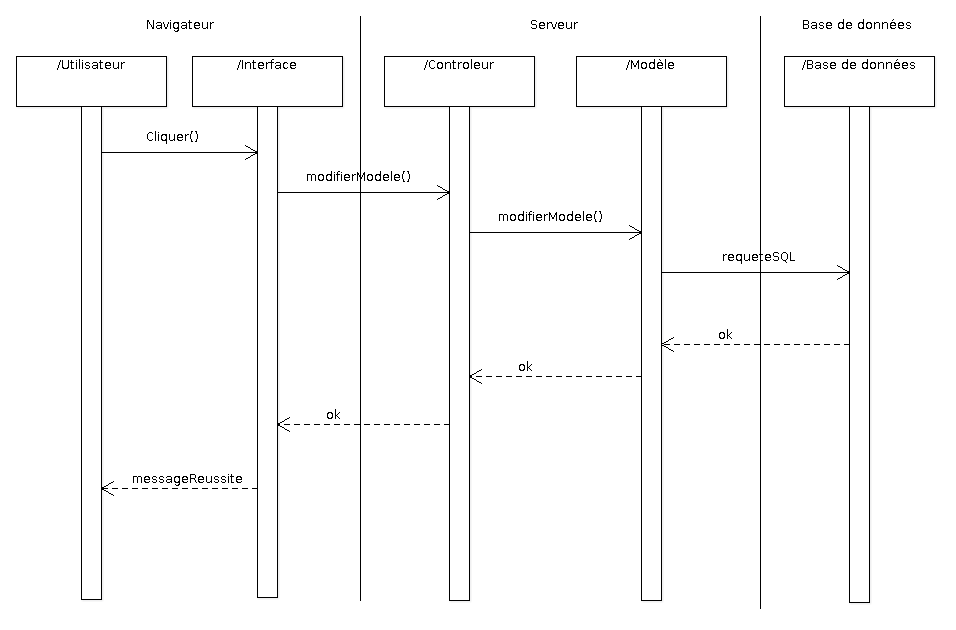
\includegraphics[scale=0.3]{diagrammeSequence/images/diagrammeSequenceAction}
	\caption{Diagramme de séquence système pour une interaction de l'utilisateur}
	\label{diagramme_sequence_2}
\end{figure}

\chapter*{Diagramme de classes}
\label{diagrammeClasse}
% version 1.00, date 20/02/16, auteur Michel Cressant
Le suivant diagramme de classe (figure \ref{diagramme_classe}) représente toutes les classes qui se retrouveront dans notre base de données finale. Cependant, pour notre premier lotissement nous nous contenterons d'implémenter les trois principales classes que sont : Benevole, Intervention et Etablissement.
\begin{figure}[H]
	\centering
	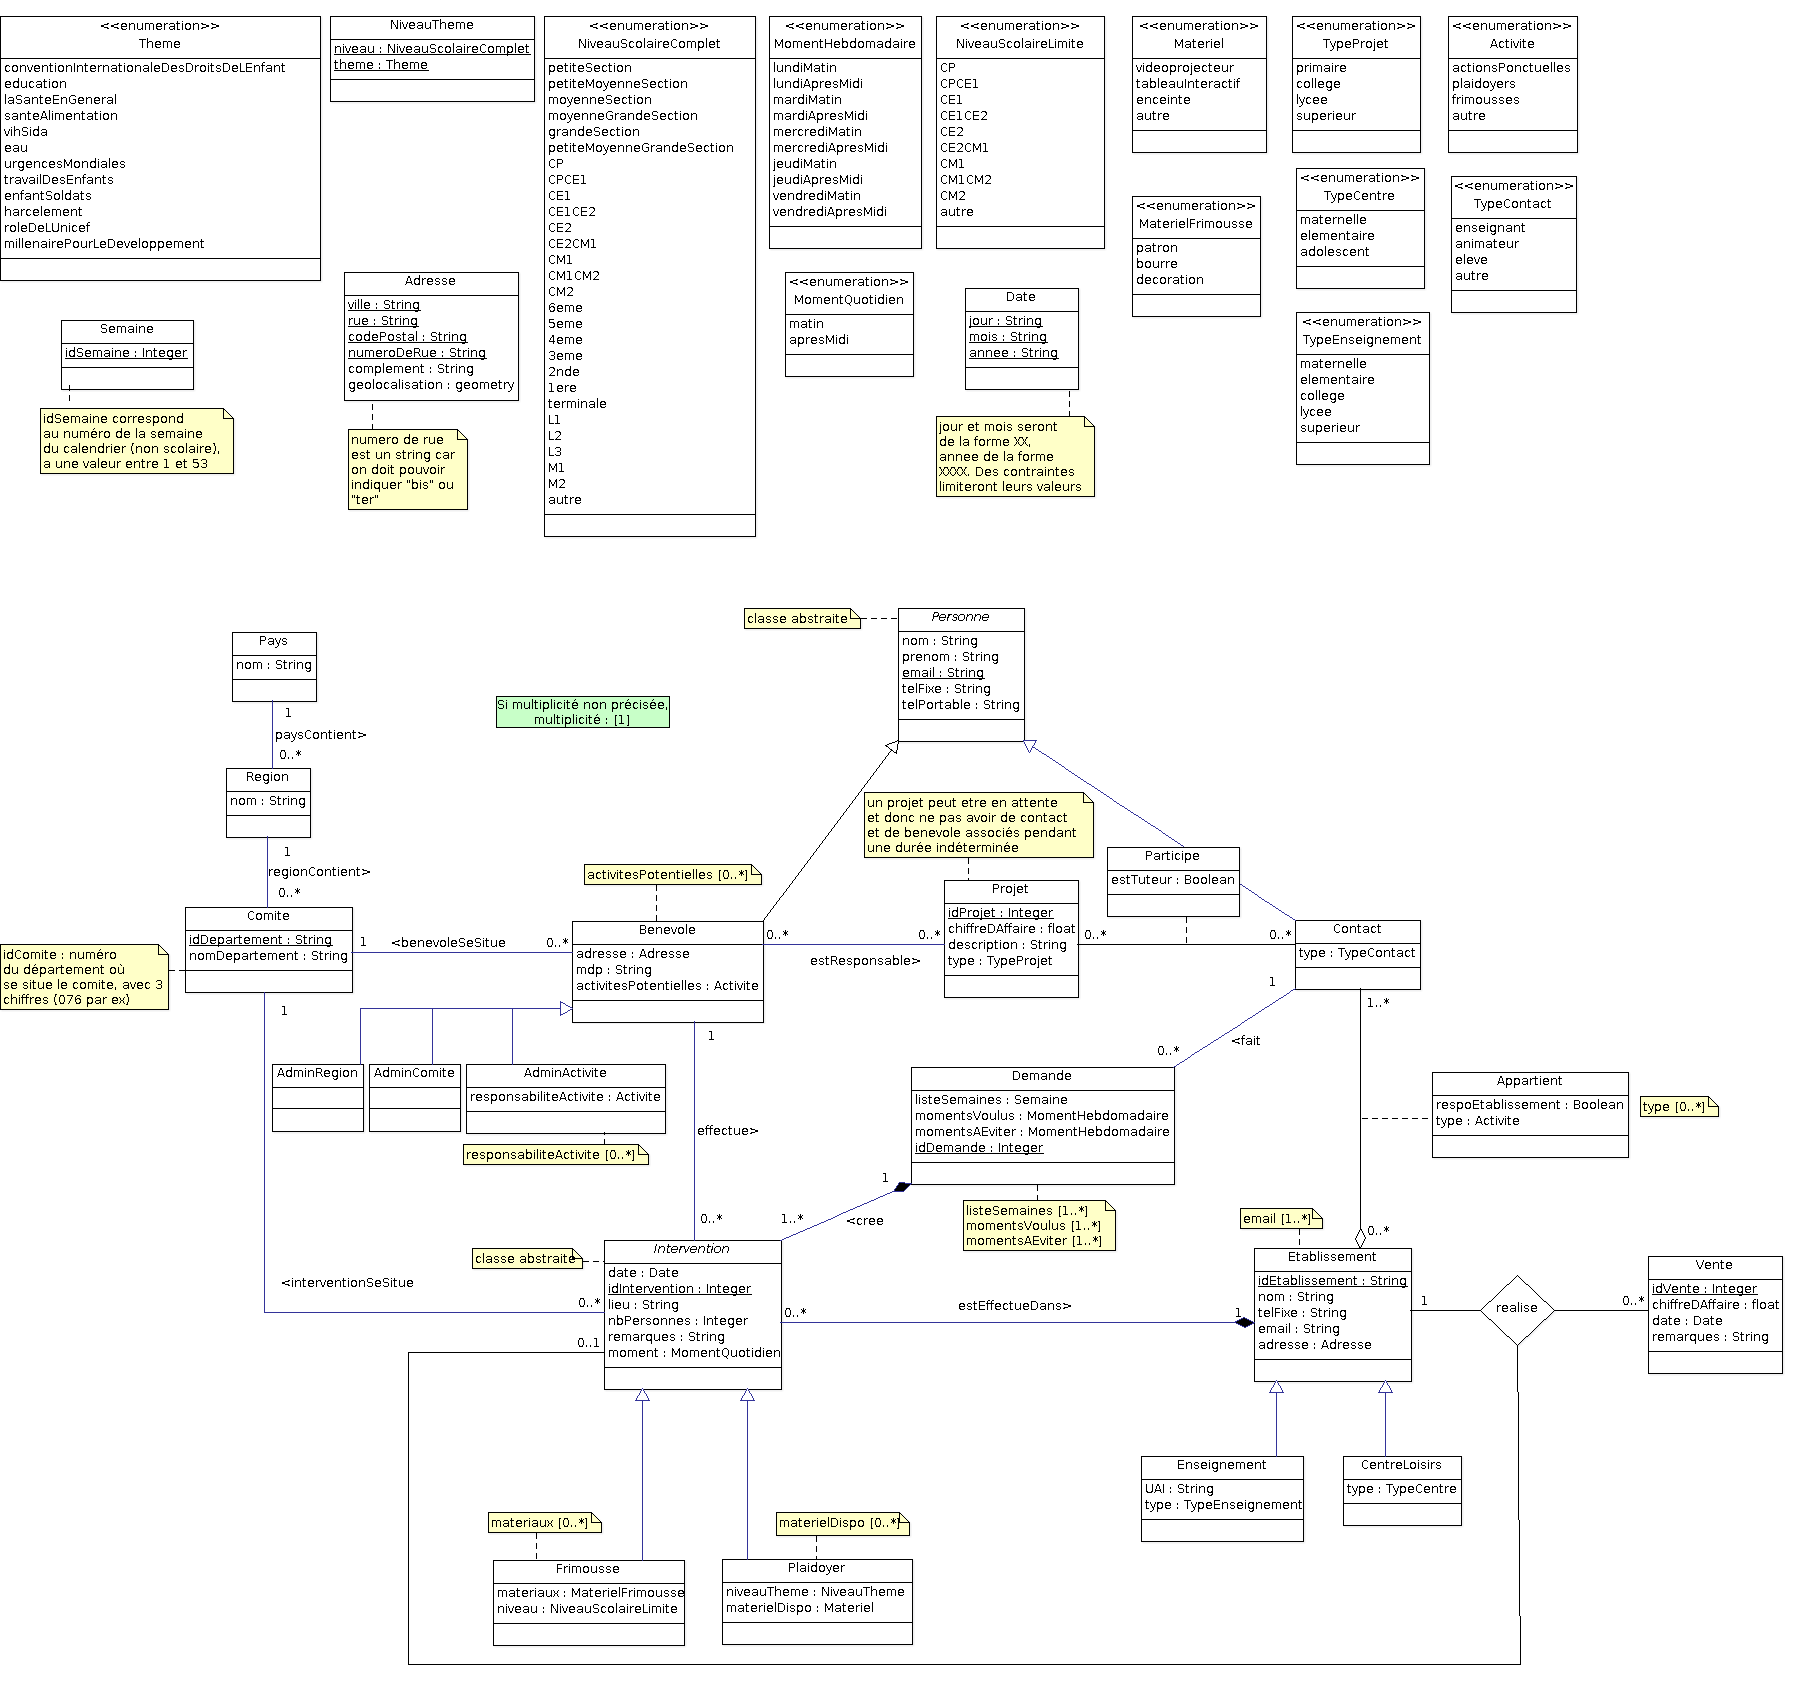
\includegraphics[scale=0.25]{diagrammeClasse/images/diagrammeDeClasses}
	\caption{Diagramme de classes}
	\label{diagramme_classe}	
\end{figure}	

\chapter*{Diagramme de packages}
\label{diagrammePackage}
\begin{figure}[H]
	\centering
	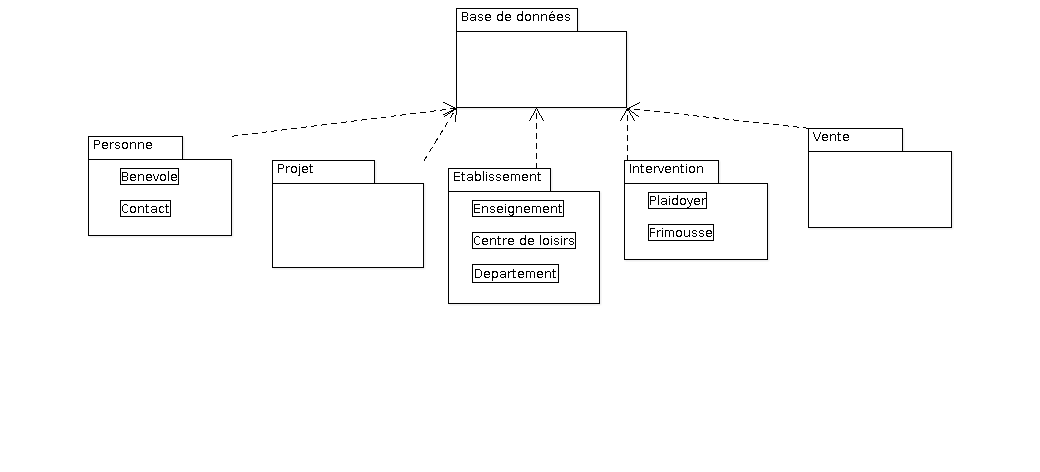
\includegraphics[scale=0.3]{diagrammePackage/images/diagrammePackage}
	\caption{Diagramme de packages}
	\label{diagramme_package}	
\end{figure}	

\begin{appendix}
\part*{Annexes}
\addcontentsline{toc}{part}{Annexes}

\listoffigures
\addcontentsline{toc}{chapter}{Table des figures}
	 
\listoftables
\addcontentsline{toc}{chapter}{Liste des tableaux}
\end{appendix}
\pageQuatriemeCouverture

\end{document}